%
% Unless otherwise indicated, the copyright in this material is 
% owned by Joerg Evermann. This material is licensed to you under the 
% Creative Commons by-attribution non-commercial license (CC BY-NC 4.0)}
%
\section*{Learning Goals}

After reading this chapter, you should be able to:
\begin{itemize}
   \item Understand the concept of tables in relational databases, including primary keys and foreign keys.
   \item Use SQL to create a set of related tables in a relational database.
   \item Understand the main elements of information retrieval from a relational database with SQL.
   \item Use SQL to filter information using the WHERE clause of a SELECT statement.
   \item Use SQL to retrieve information a set of related tables, using the JOIN clause and understand the different types of joins.
   \item Use SQL to group information using the GROUP BY and HAVING clause with different aggregation functions.
\end{itemize}

\section{Introduction}

The relational database model, developed by Edgar F. Codd in 1970, is a fundamental approach in data organization and management. It structures data in tables, or relations, comprising rows and columns, where each row signifies a record, and each column denotes a field within the record. This model is grounded in principles like tables, primary keys for unique record identification, foreign keys for inter-table relationships, and data integrity through constraints. The Structured Query Language (SQL) significantly improved the usability of data management with relational databases.

The 1970s marked the theoretical development of the relational model, focusing on data independence and efficient access. The 1980s witnessed its commercialization with the advent of relational database management systems (RDBMS) such as Oracle, IBM DB2, and Microsoft SQL Server, which became staples in enterprise applications. The 1990s saw the internet's rise bring scalability and distribution challenges to the forefront, leading to the popularity of open-source RDBMS like PostgreSQL and MySQL.

In the 2000s, with the onset of Big Data and the advent of NoSQL databases, the relational model faced new challenges. However, it continued to evolve, adapting features to handle non-relational data and integrating with cloud services. Relational databases have maintained their relevance and are extensively used in various sectors, including cloud computing, mobile applications, and big data analytics. The relational database model's focus on simplicity, flexibility, and accuracy has solidified its standing as a cornerstone in data management.

The relational database model offers several benefits and advantages, making it a popular choice for a variety of data management needs. One of its primary strengths is the simplicity of its design, which organizes data into tables, making it intuitive and easy to understand. This tabular structure facilitates efficient data retrieval and manipulation, especially with the use of SQL, a powerful and standardized query language that enhances the accessibility and handling of data.

Another significant advantage is data integrity. The relational model enforces rules through primary and foreign keys, ensuring that relationships between data are logically maintained and that the data remains consistent and accurate. This is crucial for applications where data reliability is paramount.

The model's flexibility is also a key benefit. It can easily accommodate changes in the database structure without disrupting the existing data. This adaptability makes it suitable for a wide range of applications, from small-scale projects to large, complex enterprise systems.

Moreover, relational databases support ACID (Atomicity, Consistency, Isolation, Durability) properties of transactions (that is, updates to the data), guaranteeing reliable transaction processing and robust data management, especially in multi-user environments. This ensures that even in the event of system failures or concurrent data access, the integrity of the data is maintained.

The relational model's widespread adoption has led to a rich ecosystem of tools and technologies, providing users with extensive support and resources. This includes advanced features like indexing, which enhances performance, and comprehensive security measures for data protection.

\section{Constraints and Data Types}

In relational database management systems (RDBMS), constraints are essential for ensuring the integrity of the data. Constraints can be categorized into two main types: column constraints and table constraints. Additionally, each table column is of a certain primitive data type, allowing only certain types of values to inserted. Constraints and typing ensure data quality, in that data conforms to expected rules. Table~\ref{tab:datatypes} shows an overview over commonly used datatypes. 

\begin{table}
\renewcommand{\arraystretch}{1.25}
\begin{tabularx}{\linewidth}{l|X} \hline
\textbf{Name} & \textbf{Description} \\ \hline
bigint & signed eight-byte integer \\
bit varying (\emph{varbit}) &	variable-length bit string\\
boolean & logical Boolean (true/false)\\
character varying (varchar) & variable-length character string\\
date &	calendar date (year, month, day)\\
double precision (\emph{float8}) & double precision floating-point number (8 bytes)\\
integer (\emph{int}, \emph{int4}) &	signed four-byte integer\\
interval & time span\\
\emph{json} & 	textual JSON data\\
\emph{jsonb} &	binary JSON data, decomposed\\
\emph{money} & currency amount\\
\emph{numeric} (decimal) & exact numeric of selectable precision\\
real (\emph{float4}) & single precision floating-point number (4 bytes)\\
smallint (\emph{int2}) & signed two-byte integer\\
\emph{text} &	variable-length character string\\
time & time of day (no time zone)\\
time with time zone (\emph{timetz}) & time of day, including time zone\\
timestamp & date and time (no time zone)\\
timestamp with time zone, (\emph{timestamptz}) & date and time, including time zone\\ \hline
\end{tabularx}
 (\footnotesize Source: \url{https://www.postgresql.org/docs/current/datatype.html})
\caption[Primitive Data Types in SQL and PostgreSQL]{Primitive Data Types in SQL and PostgreSQL with aliases in parentheses. \emph{Emphasized} entries are not contained in the SQL standard, they are PostgreSQL extensions.}
\label{tab:datatypes}
\end{table}

Columns constraints are rules that are applied to individual columns, while table constraints apply to combinations of columns or the entire table. Many constraints can be specified both for a single column as well as a combination of columns. 

\begin{itemize}
\item The \emph{NOT NULL}\index{Constraint!Not null}\index{Not null constraint|see{Constraint!Not null}} constraint can only be applied to individual columns and prevents NULL values from being entered into a column, ensuring that every record has a value for that column. 
\item The \emph{UNIQUE}\index{Constraint!Unique}\index{Unique constraint|see{Constraint!Unique}} constraint ensures that all values in a column are distinct, preventing duplicate entries. The UNIQUE constraint can also be used at the table level to ensure that a specific combination of values across different columns is unique for all records in the table. 
\item The \emph{CHECK}\index{Constraint!Check}\index{Check constraint|see{Constraint!Check}} constraint can be applied at the column level or at the table level. The CHECK constraint allows specifying a condition that each value in a column must satisfy. At the table level, it allows for more complex conditions that involve multiple columns. 
\item The \emph{PRIMARY KEY}\index{Constraint!Primary key}\index{Primary key constraint|see{Constraint!Primary key}} constraint is a combination of NOT NULL and UNIQUE, uniquely identifying each record in a table. The PRIMARY KEY constraints can also be applied at the table level to specify that a combination of columns uniquely identifies each record. 
\item The \emph{FOREIGN KEY}\index{Constraint!Foreign key}\index{Foreign key constraint|see{Constraint!Foreign key}} constraint is used to link columns in different tables, establishing a relationship between them. It ensures that values in a column or combination of columns must exist in the referenced colum or combination of columns. The referenced columns may be in the same table, so that the constraint expresses a \emph{unary} relationship\index{Unary relationship}, or in another table, so that the constraint expresses a \emph{binary} relationship\index{Binary relationship}. Together with NOT NULL constraints, this allows the repsentation of optional or mandatory relationships. 
\end{itemize}

\section{Introduction to SQL and PostgreSQL}

Despite its name, SQL\index{Structured query language}\index{SQL|see{Structured query language}} serves as a language not only for querying but for data definition, data manipulation, data access control, transaction control, and querying. SQL has been standardized by the American National Standards Institute (ANSI) and the International Organization for Standardization (ISO), ensuring a consistent syntax and set of features across different database systems. However, many database systems extend standard SQL with proprietary extensions to enhance functionality and performance. Despite these variations, the core elements of SQL remain widely consistent, contributing to its status as the lingua franca of database management. 

This section covers only the most basic aspects of SQL, insofar as they are necessary to understand the relational database schema and to use SQL to query data for descriptive data analytics. The most important SQL commands are listed in Table~\ref{tab:sql}. For more further information, consult the relevant sections of the PostgreSQL documentation on data definition\footnote{\url{https://www.postgresql.org/docs/current/ddl.html}}, data manipulation\footnote{\url{https://www.postgresql.org/docs/current/dml.html}}, data queries\footnote{\url{https://www.postgresql.org/docs/current/queries.html}} and primitive data types\footnote{\url{https://www.postgresql.org/docs/current/datatype.html}}.

\begin{table}
\renewcommand{\arraystretch}{1.25}
\centering

\begin{tabular}{l|l} \hline
CREATE TABLE & Create a new table with specified columns and constraints \\ 
DROP TABLE & Deletes a table and all its contents \\
INSERT & Inserts a row of data values into a table \\
UPDATE & Updates/modifies data values in a table \\
SELECT & Retrieves data values from one or more tables \\ \hline
\end{tabular}
\caption{Basic SQL Commands}
\label{tab:sql}
\end{table}

\begin{wrapfigure}{l}{1in}
\begin{center}
\includegraphics[height=.5in]{postgresql-logo.png}
\end{center}
\end{wrapfigure}

The PostgreSQL RDBMS (relational database management system) is installed in the course virtual machine or can be downloaded from the PostgreSQL website\footnote{\url{https://www.postgresql.org/download/}}. A DBMS is typically a background computer application without a user interface. It is typically used by other computer applications, such as accounting software to store financial information, a logistics management software to store information about shipments, a customer relationship management system to store information about customers and marketing campaigns, etc. 

End users can interact with a DBMS using administration software, such as the basic ''psql'' command line software or a graphical application like ''pgAdmin'' or ''DBeaver''. The desktop version of pgAdmin and DBeaver are installed in the course virtual machine, or can be downloaded from their websites\footnote{\url{https://www.pgadmin.org/download/}, \url{https://dbeaver.io/download/}}. They provide easy-to-use tools for creating tables and querying data, but this section focuses on using the SQL language instead.

A DBMS runs on a single computer (''server'') or, if the amount of data is very large, distributes the data across a cluster of multiple computers. Different DBMS differ in their performance, the ease with which data can be distributed, and the scalability to very large clusters. However, from the users perspective, these technical considerations are largely invisible. \emph{When connecting to a DBMS that runs on your own computer, use the computer name ''localhost''}.

A DBMS can manage multiple databases\index{Database management system}\index{DBMS|see{Database management system}}. \emph{A database named ''busi4720'' has already been created in your course virtual machine, using the CREATE DATABASE command}. pgAdmin and DBeaver also have the ability to show the SQL command that creates every element in a DBMS, including databases, tables, and constraints. This is useful to understand exactly what elements are contained in a database or in a table and any constraints imposed upon them.

Every database can have multiple schema\index{Schema!in relational database}. A schema is a collection of tables with their columns and constraints, as well as related elements such as functions, procedures, triggers, views and others. In PostgreSQL, every database contains the schema ''public''. This is the default schema and is used when no other schema is specified. 

\begin{figure}
\centering
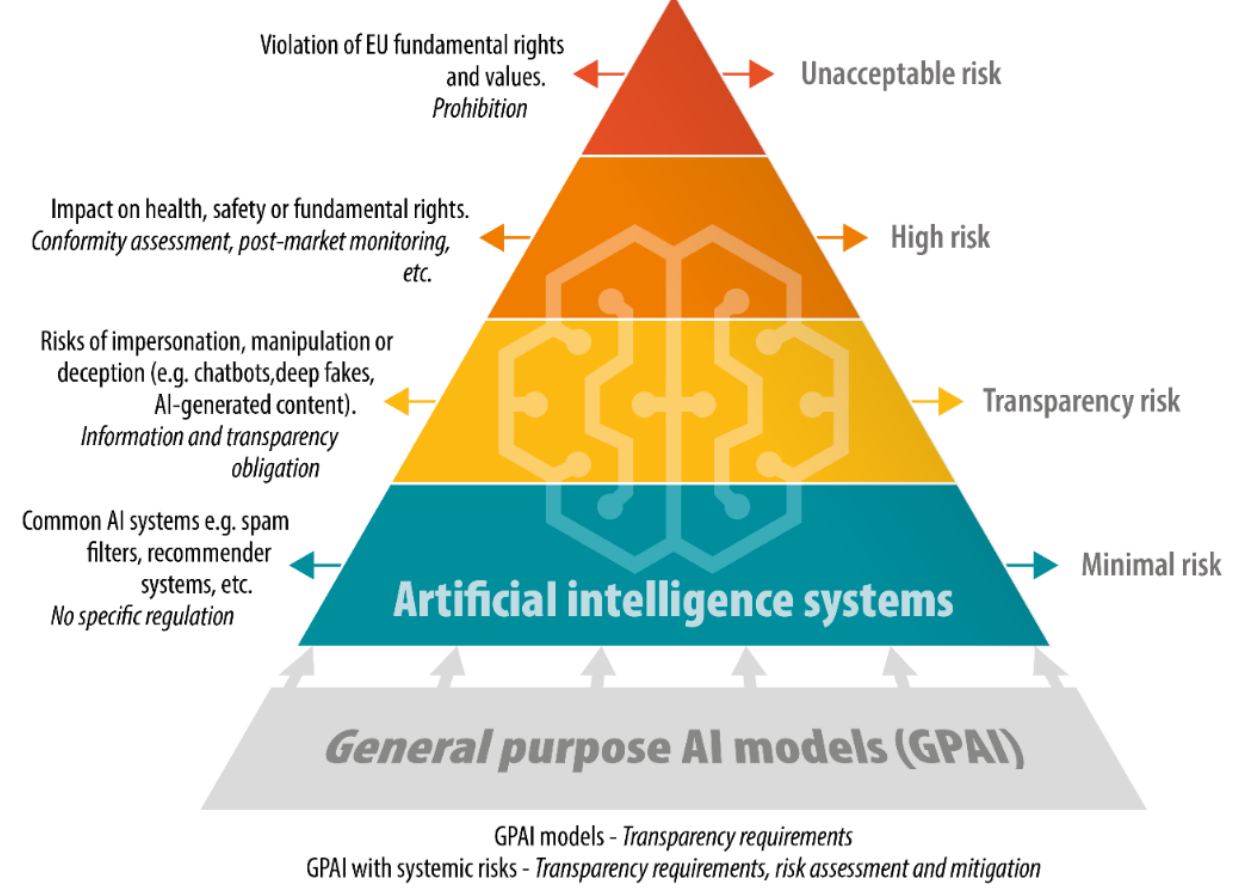
\includegraphics[width=.9\textwidth]{screen2.png}
\caption{pgAdmin Query tool}
\label{fig:querytool}
\end{figure}

When the pgAdmin application is initially launched, it will connect to the DBMS that is running on the local machine (''localhost'') with the username ''busi4720'' (its password is ''busi4720'') and will show an ''Object Explorer'' in the left part of the application. This allows navigation and exploration of the contents of this DBMS, as shown in Figure~\ref{fig:querytool}.

\begin{figure}
\centering
\includegraphics[width=.9\textwidth]{screen4.png}
\caption{DBeaver database tool}
\label{fig:dbeaver}
\end{figure}

Similarly, when the DBeaver application is first started, it will also conncect to the DBMS that is running on the local machine and will show a ''Database Navigator'' in the left part of the application window (Figure\ref{fig:dbeaver}. Navigate the contents of the DBMS to the ''busi4720'' database and the ''public'' schema.

\begin{figure}
\centering
\includegraphics[width=.9\textwidth]{screen3.png}
\caption{psql command line tool}
\label{fig:psql}
\end{figure}

The basic ''psql'' command line tool can be started by by typing \texttt{psql} into a terminal window. The course virtual machine is configured to provide automatic access to the ''busi4720'' database. The database connection can be confirmed by executing the \texttt{\textbackslash conninfo} command in psql. Use psql options to specify other connections using the template \texttt{psql -d dbname -h hostname -u username}. Figure~\ref{fig:psql} shows the psql command line tool in a terminal window.

\begin{alertbox}
\noindent \emph{The examples and exercises in the remainder of this chapter refer to the ''busi4720'' database.}
\end{alertbox}

\section{Data Definition in SQL}

\begin{infobox}
SQL commands are traditionally written in upper case letters and this is done here as well. However, SQL is not case sensitive, so that capitalization does not actuallly matter. Traditionally, an SQL command must end with a semicolon. This is done here as well, although some DBMS may no longer require this. 
\end{infobox}

For this example, assume that your database will be used to store information about products. The CREATE TABLE data definition command in SQL\index{Data definition language!SQL} is used to create tables, their columns, and constraints. This first example creates a simple table with three columns to store product data.

\begin{sqlcode}
CREATE TABLE products (
  pcode integer,
  name  varchar(100) NOT NULL,
  price float4,
  PRIMARY KEY (pcode) 
);
\end{sqlcode}

\begin{infobox}
To run this code, enter it into psql or the SQL code windows of pgAdmin or DBeaver. Then,
\begin{itemize}
   \item in psql, press \colorbox{lightgray}{RETURN} to execute
   \item in DBeaver, press \colorbox{lightgray}{CTRL-RETURN} to execute
   \item in pgAdmin, press \colorbox{lightgray}{F5} to execute.
\end{itemize}
\end{infobox}

The table contains a column named ''pcode'' (to store the product code) that is of integer type, that is, it can contain whole numbers only. The table has a column called ''name'' of characters with a varying length and a maximum length of 100 characters to store product names. Additionally, a column NOT NULL constraint has been defined for this column, ensuring that a name always exists for a product. The table has a column named ''price'' that is of a single precision floating point type (4 bytes), that is, it can hold decimal point numbers to store product prices. The final line of the SQL command created a primary key constraint on the single column ''pcode'' to ensure that the product code must not be NULL and must be unique, ensuring that each row in the table represents a distinct product. Note that column ''price''may be NULL, that is, may not contain values, because no NOT NULL constraints have been specified. This may be useful for example when the price has not been decided on or will be calculated later.

The following SQL code block creates a table for suppliers. The table has a similar structure to the products table and similar NOT NULL and PRIMARY KEY constraints.

\begin{sqlcode}
CREATE TABLE suppliers (
  scode integer,
  name  varchar(100) NOT NULL,
  city  varchar(100),
  PRIMARY KEY (scode) 
);
\end{sqlcode}

After creating tables with the data definition part of the SQL language, the data manipulation commands of SQL can be used to insert or update values in the tables. The following SQL code block inserts two rows into each of the tables that were just created. Enter the following SQL commands in the Query tool:

\begin{sqlcode}
INSERT INTO products VALUES (1, 'Hex Bolt', 1.99);
INSERT INTO products VALUES (2, 'Round Bolt', 2.99);

INSERT INTO suppliers VALUES (1, 'Bolts Inc', 'HVGB');
INSERT INTO suppliers VALUES (2, 'Hardware Co', 'Cartwright');
\end{sqlcode}

The values for each row must be specified in the order in which the columns of the table are defined. For the ''products'' table this is first the product code, followed by the name, and finally the price. For the ''suppliers'' table, this is first the supplier code, then the name and then the city. There are many different variations on the basic INSERT statement; consult the official documentation using the links in the earlier footnote.

After inserting the values, a basic SELECT statement, which is the core querying command in SQL, checks that the data is actually in the tables. Run the commands in the following SQL code block one at a time to see each command's results:

\begin{sqlcode}
SELECT * FROM products;
SELECT * FROM suppliers;
\end{sqlcode}

This is the simplest form of a SELECT statement, the asterisk (''*'') instructs SQL to retrieve all columns. Later examples will illustrate ways to retrieve only some columns, and many other variants on the SELECT statement.

The two tables allow capturing information about products and information about suppliers, but they do not allow capturing which supplier supplies which product. In order to do this, the two tables need to be related by a foreign key relationship. 

For the following example, assume that suppliers can supply many products, but a product may be supplied by only one supplier (or no supplier at all). This is called a \emph{one-to-many relationship}. The following SQL code block alters the tables, retaining the existing data, and then updates the information in the new ''supplier'' column for the ''products'' table:

\begin{sqlcode}
ALTER TABLE products ADD COLUMN supplier integer;
ALTER TABLE products ADD FOREIGN KEY (supplier) REFERENCES suppliers;

UPDATE products SET supplier = 1 WHERE pcode = 1;
UPDATE products SET supplier = 1 WHERE pcode = 2;
\end{sqlcode}

The first SQL statement above adds a new column to the existing products table in which to record the supplier of the product. The second line creates a foreign key reference from the supplier column in the products table to the primary key of the suppliers table; the primary is the ''scode'' column (see SQL code above). This ensures that only those suppliers can be recorded in the products table that actually exist in the suppliers table. 

The third and fourth line update the data in the products table and set the value of the supplier column for different products. The two products have the same supplier which reflects the assumption that a supplier may supply multiple products. On the other hand, only one supplier can be recorded for each product, and this too reflects the above assumption. This expresses the \emph{one-to-many relationship}. Moreover, the value of the supplier column in the products table may be NULL. In fact, after altering the table to add this column, all its values were NULL. A NULL value reflects the fact that a product has no supplier.

As an alternative to altering the existing products table, drop the products table to delete it and re-create it. Then insert some values. The following SQL code block uses the DROP TABLE command of SQL to delete the products table and all its contents.

\begin{sqlcode}
DROP TABLE products;

CREATE TABLE products (
  pcode    integer,
  name     varchar(100),
  price    float4,
  supplier integer,
  PRIMARY KEY (pcode),
  FOREIGN KEY (supplier) REFERENCES suppliers 
);
  
INSERT INTO products VALUES(1, 'Hex Bolt', 1.99, 1);
INSERT INTO products VALUES(2, 'Round Bolt', 2.99, 1);
INSERT INTO products VALUES(3, 'Square Bolt', 3.99, NULL);
\end{sqlcode}

The above SQL code achieves the same as altering the table but in the process deletes all data in the products table. When possible, it is therefore preferable to use multiple ALTER TABLE statements instead of DROP and CREATE statements. 

Note the following important points about the tables so far:
\begin{itemize}
  \item There are products that have no supplier (the ''square bolt'')
  \item There are suppliers that supply many products (supplier 1)
  \item There are suppliers that do not supply products (supplier 2)
\end{itemize}

In the products table as altered or re-created to this point, it is possible that a product has no supplier. However, in some applications it may be necessary to enforce that it is mandatory for products to have a supplier. This is done by adding a NOT NULL constraint, either by altering the table again, as in the following SQL code block, or by re-creating it with the appropriate constraint added.

\begin{sqlcode}
ALTER TABLE products ALTER COLUMN supplier SET NOT NULL;
\end{sqlcode}

Adding constraints can only be done when the constraint is already satisfied. This means that in this example, none of the values of the supplier columns can be NULL when adding the constraint. If a new constraint is violated, the DBMS will show an error and the constraint will not be added.

When re-creating the table, the NOT NULL column constraint can be defined in the CREATE TABLE statement:

\begin{sqlcode}
DROP TABLE IF EXISTS products;

CREATE TABLE products (
  pcode    integer,
  name     varchar(100),
  price    float4,
  supplier integer NOT NULL,
  PRIMARY KEY (pcode),
  FOREIGN KEY (supplier) REFERENCES suppliers 
);
\end{sqlcode}

So far, the assumption was that each product can has one supplier. However, in many settings, products have multiple suppliers, and suppliers supply multiple products, that is, there is a \emph{many-to-many relationship} between the two. Expressing many-to-many relationships requires a third table that explicitly represents the relationship, here the ''supplies'' relatinship between products and suppliers. The following SQL code first removes the existing tables, then re-creates tables to express a many-to-many relationship instead.

\begin{sqlcode}
DROP TABLE IF EXISTS products;
DROP TABLE IF EXISTS suppliers;

CREATE TABLE products (
  pcode integer,
  name  varchar(100),
  PRIMARY KEY (pcode) );

CREATE TABLE suppliers (
  scode integer,
  name  varchar(100),
  city  varchar(100),
  PRIMARY KEY (scode) );
  
CREATE TABLE supplies (
  scode  integer NOT NULL,
  pcode  integer NOT NULL,
  price  float4 NOT NULL,
  PRIMARY KEY (scode, pcode),
  FOREIGN KEY (scode) REFERENCES suppliers,
  FOREIGN KEY (pcode) REFERENCES products );
\end{sqlcode}

Note that the tables must be dropped in the right order: ''products'' first, then ''suppliers'' because the products depend on the suppliers due to the foreign key constraint\footnote{Use the CASCADE keyword to drop dependent tables automatically but use with care.}. The IF EXISTS part is a safeguard to prevent an error if the table does not exist when attempting to drop it.

The primary key of the supplies table is a \emph{compound key}\index{Compound key}, that is, it consists of a combination of columns. The supplies table is related by two FOREIGN KEY constraints both to the products and suppliers table so that only products and suppliers that already exist can be recorded here (and thereby related to each other). The price column is no longer in the products table, but has been moved to the supplies table, because each supplier may supply a product at a different price. The following example data shows this:

\begin{sqlcode}
INSERT INTO products VALUES (1, 'Hex Bolt');
INSERT INTO products VALUES (2, 'Round Bolt');

INSERT INTO suppliers VALUES (1, 'Bolts Inc', 'HVGB');
INSERT INTO suppliers VALUES (2, 'Hardware Co', 'Cartwright');

INSERT INTO supplies VALUES(1, 1, 1.99);
INSERT INTO supplies VALUES(1, 2, 2.49);
INSERT INTO supplies VALUES(2, 1, 2.99);
INSERT INTO supplies VALUES(2, 2, 1.79);
\end{sqlcode}

\noindent To clean up after these exercises, drop all tables if they are no longer required:

\begin{sqlcode}
DROP TABLE supplies;
DROP TABLE products;
DROP TABLE suppliers;
\end{sqlcode}

\paragraph*{Summary} In summary, a \emph{one-to-many relationships} requires a foreign key from the ''many'' table that references the ''one'' table and its primary key. In the first example above, a supplier supplies many products but a product has one supplier (or none, depending on whether a NOT NULL constraint has been specified). In contrast, a \emph{many-to-many relationship} requires a table that explicitly represents the relationship. Foreign keys from this table reference the participating, original, ''main'' tables and their primary keys. In the second example above, a supplier supplies many products and a product can be supplied by many suppliers. 

In fact, this type of relationship can be extended in a straightforward way to three or more tables. For example, a supplier supplies many products from many warehouses, a product may be supplied by many suppliers from many warehouses, and a warehouse may contain many products from many suppliers. 

\begin{exercisebox}
\begin{enumerate}
  \item Consider the following information:
	\begin{itemize}
	  \item A book has an ISBN number and a title. 
	  \item An author has a name and an address. 
	  \item An author can write many books, and a book can be written by multiple authors. A book is written in a certain year.
	\end{itemize}
  \item Write the CREATE TABLE statements with the necessary FOREIGN KEY statements, and execute them on PostgreSQL
  \begin{itemize}
    \item Use appropriate datatypes for the columns
    \item Create an appropriate PRIMARY KEY for all tables
  \end{itemize}
  \item Use INSERT statements to create some example data.
  \item Use SELECT statements to ensure your data exists.
\end{enumerate}
\end{exercisebox}

\section{SQL Queries}

\subsection*{Basic Queries with the SELECT Statement}

The SELECT statement in SQL is used to query and retrieve data from one or more tables in a database. The basic structure of a SELECT statement allows specification of which columns of data you want to retrieve and from which tables. A SELECT statement has multiple clauses or parts that are used to specific different characteristics of the information to retrieve:

\begin{itemize}
 \item \texttt{SELECT}: Which columns to query (use the asterisk ''\texttt{*}'' to select all).
 \item \texttt{FROM}: Which tables to query from.
 \item \texttt{JOIN}: How to combine data from multiple tables based on related columns.
 \item \texttt{WHERE}: Conditions on field values used to filter the retrieved records.
 \item \texttt{GROUP BY}: Groups within which to aggregate data using an aggregate function such as \texttt{sum()}, \texttt{count()}, or \texttt{max()}.
 \item \texttt{HAVING}: Conditions on group aggregate values. Similar to WHERE but for aggregates within each group.
 \item \texttt{ORDER BY}: How to sort the resulting records in either ascending or descending order.
 \item \texttt{LIMIT}: Limit on how many results to return.
\end{itemize}

To demonstrate the basic use of SQL queries to retrieve information from a relational database, it is best to begin with a simple example, that of the 1:Many relationship between products and suppliers set up earlier. The following SQL commands (re-)create this example with a few more rows of data in the products table:

\begin{sqlcode}
-- Drop tables if they exist
DROP TABLE IF EXISTS products;
DROP TABLE IF EXISTS suppliers;

-- Set up tables with 1:Many relationship:
CREATE TABLE suppliers (
scode integer,
name varchar(100),
city varchar(100),
PRIMARY KEY (scode) );

CREATE TABLE products (
pcode	integer,
name	varchar(100),
price	float4,
scode   integer,
PRIMARY KEY (pcode),
FOREIGN KEY (scode) REFERENCES suppliers );
\end{sqlcode}

\begin{sqlcode}
-- Insert some data:
INSERT INTO SUPPLIERS VALUES (1, 'Bolts Inc', 'HVGB');
INSERT INTO SUPPLIERS VALUES (2, 'Hardware Co', 'Cartwright');

INSERT INTO products VALUES(1, 'Hex Bolt A', 1.99, 1);
INSERT INTO products VALUES(2, 'Round Bolt 1', 2.99, 1);
INSERT INTO products VALUES(3, 'Square Bolt B', 3.99, 1);
INSERT INTO products VALUES(4, 'Hex Bolt B', 2.99, 1);
INSERT INTO products VALUES(5, 'Round Bolt 2', 1.99, 2);
INSERT INTO products VALUES(6, 'Square Bolt 7', 3.49, 2);
\end{sqlcode}

With this data, the simplest SQL query contains only the SELECT and the FROM clauses to retrieve a set of columns from a single table. The following SQL code uses the asterisk (''\texttt{*}'') to select all columns and returns all rows from the products table:

\begin{sqlcode}
SELECT * FROM products;
\end{sqlcode}

The WHERE clause filters the selected rows. The next example returns only products for supplier 1, that is, those rows in the products table where ''scode=1''. Multiple conditions can be surrounded in parentheses and combined with the keywords AND and OR.

\begin{sqlcode}
SELECT * FROM products WHERE scode = 1;
\end{sqlcode}

The following SQL code selects only a few named columns from the products table and also filters the retrieved rows by price:

\begin{sqlcode}
SELECT name, supplier FROM products WHERE price < 3;
\end{sqlcode}

The ORDER BY clause is used to order the result, possibly by using multiple columns and with specified ascending or descending direction. The following SQL code block selects all columns and returns all rows from the products table ordered first ascending by price, and then, when the price is the same, descending by name:

\begin{sqlcode}
SELECT * FROM products ORDER BY price ASC, name DESC;
\end{sqlcode}

The LIMIT clause can be used to limit the number of returned rows. This is often useful in combination with the ORDER BY clause to select the largest or smallest values. The following example demonstrates this by retrieving the name of the cheapest three products from the products table:

\begin{sqlcode}
SELECT name FROM products ORDER BY price ASC LIMIT 3;
\end{sqlcode}

The JOIN clause combines information from two or more tables. This is done by specifying either a common column, or an explicit join condition if the corresponding column names in the two tables are different. The following SQL code shows an example of retrieving all columns from the products table and their corresponding rows from the suppliers table using an INNER JOIN clause USING the common column ''scode'':

\begin{sqlcode}
SELECT * FROM products INNER JOIN suppliers USING (scode);
\end{sqlcode}

If multiple common columns are needed to find corresponding rows, they can be specified in parentheses simply be expanding the above example of the USING clause.

The following two SQL expressions are essentially equivalent to the one above and to each other. Instead of the USING clause for common columns, the first expression explicitly specifies the join condition with the ON clause, while the second expression completely omits the JOIN clause and instead specifies both tables in the FROM clause and uses a condition in a WHERE clause to select corresponding rows in the two tables:

\begin{sqlcode}
-- (Almost) Equivalent:
SELECT * FROM products 
    INNER JOIN suppliers ON products.scode=suppliers.scode;

SELECT * FROM products, suppliers 
    WHERE products.scode=suppliers.scode;
\end{sqlcode}

In the above JOIN examples, both the products and suppliers table contain a column ''name''. It is often useful to rename columns for clarity. The following example shows how this can be done using the AS keyword. It also demonstrates how the ambiguity of columns with the same name in different tables can be resolved by using the form ''table.column'' to select columns:

\begin{sqlcode}
-- Rename columns for clarity:
SELECT products.name AS "Product", 
       price AS "Price", 
       suppliers.name AS "Supplier", 
       city AS "Location"
    FROM products INNER JOIN suppliers USING (scode);
\end{sqlcode}

The previous two examples used the ''INNER JOIN'', the most commonly used type of join between two tables. Table~\ref{tab:sqljoins} shows a list of other possible join types. 

The INNER JOIN selects only those rows that have a corresponding row or rows in the other table, and vice versa. The LEFT OUTER join selects all rows from table T1, even those that do not have a corresponding row in table T2. For the missing corresponding rows, it simply returns NULL values. The RIGHT OUTER join does the same thing but from the perspective of table T2. That is, it returns all rows of T2, but for those rows that do not have a corresponding entry in table T1, it returns NULL values. The FULL OUTER join is a combination of the LEFT OUTER and RIGHT OUTER joins.

\begin{table}
\centering

\renewcommand{\arraystretch}{1.5}
\small
\begin{tabularx}{.8\textwidth}{l|X} \hline
INNER & Selects only rows from T1 that have corresponding row in T2 and vice versa. \\
LEFT OUTER & Selects all rows from T1, if T2 does not have a corresponding row, NULL values are inserted. \\
RIGHT OUTER & Select all rows from T2, if T1 does not have a corresponding row, NULL values are inserted. \\
FULL OUTER & Selects all rows from T1, T2. If the other table is missing corresponding row, NULL values are inserted. \\ \hline
\end{tabularx}

\caption{Types of Joins between two tables T1 and T2 in SQL}
\label{tab:sqljoins}
\end{table}

The GROUP BY clause of an SQL query is used in combination with aggregate functions for grouping information and calculating aggregate values. The easiest aggregation is to simply count the number of rows or entries for each group using the ''count(.)'' function, shown in the first example that selects the number of products for each supplier, that is, the count of rows in table products grouped by supplier code:

\begin{sqlcode}
-- Select the number of products for each supplier
SELECT scode, count(*) from products GROUP BY scode;
\end{sqlcode}

To also include the names of the suppliers requires joining the suppliers table, as shown below:
\begin{sqlcode}
-- Add the name of suppliers by joining suppliers table
SELECT suppliers.name, count(*)
    FROM suppliers INNER JOIN products USING (scode)
    GROUP BY scode;
\end{sqlcode}

The SQL code below illustrates another aggregate function, the average (''AVG'') and also shows that the aggregates can be used in the ORDER BY clause. The query returns the mean price of products for each suppliers, ordered descending by mean price:

\begin{sqlcode}
-- Mean price of products for each supplier, ordered descending
SELECT suppliers.name, AVG(price)
    FROM suppliers INNER JOIN products USING (scode)
    GROUP BY scode
    ORDER BY AVG(price) DESC;
\end{sqlcode}

Finally, the HAVING clause is a filter clause like the WHERE clause, but instead of filtering the rows in a table, it filters the groups in a GROUP BY clause. The following SQL query returns only suppliers for which the average price of their products is less than 2.8:

\begin{sqlcode}
-- Find only suppliers for which average price less than 2.80:
SELECT suppliers.name, AVG(price)
    FROM suppliers INNER JOIN products USING (scode)
    GROUP BY scode
    HAVING AVG(price) < 2.8;
\end{sqlcode}

Besides COUNT() and AVG() functions, SQL provides other aggregate functions, shown in Table~\ref{tab:sqlaggregates}. However, many of these are specific to various relational database management systems, like PostgreSQL. 

\begin{table}
\centering

\renewcommand{\arraystretch}{1.5}
Standard SQL: \\

\small
\begin{tabular}{l|l|l|l|l} \hline
\
MIN() & MAX() & COUNT() & SUM() & AVG() \\ \hline
\end{tabular}

\normalsize

\vspace{\baselineskip}
PostgreSQL (excerpt):\\

\small
\begin{tabular}{l|l|l} \hline
CORR() & STDDEV() & VARIANCE() \\
MODE() & PERCENTILE() & REGR\_SLOPE() \\
REGR\_R2() & RANK() & DENSE\_RANK() \\ \hline
\end{tabular}

\caption{Frequently Used Aggregation Functions}
\label{tab:sqlaggregates}
\end{table}

\noindent To clean up after these exercises, drop all tables if they are no longer required:

\begin{sqlcode}
DROP TABLE products;
DROP TABLE suppliers;
\end{sqlcode}

\subsection*{Relational Diagrams}

The previous section has presented the basics of the relational database model, focusing on how tables are related by foreign key relationships. Tables and their relationships are often graphically shown in a \emph{relational diagram}\index{Relational diagram}. Such diagrams are often called ''\emph{ER Diagrams}\footnote{Technically, the two are not quite the same.}''\index{ER diagram|see{Entity-relationship diagram}} or ''Entity-Relationship Diagrams''\index{Entity-relationship diagram}. A graphical representation of the database structure is useful for understanding the data and for writing queries to extract data from the table or tables of the database. 

In many software tools, including in pgAdmin, the database developer can use relational diagrams to create tables, instead of writing CREATE TABLE statements. In the reverse, relational diagrams can also be automatically created from an existing database and its tables. 

\begin{exercisebox}In the pgAdmin Object Explorer, right-click on the ''busi4720'' database, then select ''ERD for Database'' to create a relational diagram. \\

In the DBeaver Database Navigator, select the ''busi4720'' database, then right-click on its ''public'' schema and select ''View Diagram'' to create the diagram.
\end{exercisebox}

\noindent The resulting diagram will look similar to the one in Figure~\ref{fig:pagila}. (If you did not clean up the tables you created in the above SQL exercises, these will be present in the diagram as well).

\begin{figure}
\centering

\includegraphics[width=.95\textwidth]{pagila2dbeaver.png}
\caption{Relational diagram of the Pagila demo database}
\label{fig:pagila}
\end{figure}


\subsection*{The Pagila Database}

The diagram shows the structure of the \emph{Pagila} database\footnote{\url{https://github.com/devrimgunduz/pagila}, \\
\url{https://github.com/devrimgunduz/pagila/blob/master/LICENSE.txt}}, a demonstration database originally developed for teaching and development of the MySQL RDBMS under the name Sakila\footnote{\url{https://dev.mysql.com/doc/sakila/en/}, \\
\url{https://dev.mysql.com/doc/sakila/en/sakila-license.html}}. Pagila is designed as a sample database to illustrate database concepts and is based on a fictional DVD rental store. It consists of multiple tables for film and actor information, customer data, store inventory, and rental transactions. Here is an overview of the key tables in the Pagila database:

\begin{itemize}
  \item \emph{actor}: Stores details about actors, including their first and last names.
  \item \emph{film}: Contains information about movies, such as title, release year, language, rental duration, rental rate, length, replacement cost, rating, and special features.
  \item \emph{film\_actor}: A junction table that establishes a many-to-many relationship between the films and actors. It links each film to its actors.
  \item \emph{category}: Lists different genres or categories of films.
  \item \emph{film\_category}: Another junction table that connects films to their respective categories.
  \item \emph{language}: Stores languages in which the films are available.
  \item \emph{customer}: Contains customer information, including names, email addresses, addresses, and store ID where they are registered.
  \item \emph{address}: Holds address details, including city, postal code, phone number, and other address components.
  \item \emph{city}: Contains information about cities, linked to the addresses.
  \item \emph{country}: Stores country information, which is linked to cities.
  \item \emph{store}: Includes data about the DVD rental stores, such as the store's address and the staff.
  \item \emph{inventory}: Contains information about the store's inventory, including which film copies are available at which store.
  \item \emph{rental}: Records details about rental transactions, including rental and return dates, inventory, and customer information.
  \item \emph{payment}: Tracks payments made by customers for rentals, including amount and payment date.
  \item \emph{staff}: Contains information about the store staff, including their names, email addresses, and the store they work in.
\end{itemize}

Each table is designed with primary keys for unique identification and foreign keys to establish relationships with other tables. This structure allows for complex queries across multiple tables, facilitating a wide range of analyses, from inventory management to customer behavior tracking. The Pagila database is a good example of a real-world database schema and offers a good data set for practicing SQL queries.

\subsection*{Advanced SQL Query Examples}

The following examples show queries for the Pagila database to illustrate different features of the SELECT statement. Instead of describing every option in detail, to understand SQL it is useful to execute the queries and learn by modifying the queries and observing changes in the results. 

\paragraph{Example:} Find all actors and the films they appeared in, ordered by film category and year, for those films that are rated PG

\begin{sqlcode}
SELECT concat(left(actor.first_name, 1), '. ', 
           actor.last_name) AS Actor, 
       category.name AS Category, 
       film.title, 
       film.release_year
  FROM film_actor
  INNER JOIN actor USING (actor_id)
  INNER JOIN film USING (film_id)
  INNER JOIN film_category USING (film_id)
  INNER JOIN category USING (category_id)
  WHERE film.rating = 'PG'
  ORDER BY actor.last_name, 
           actor.first_name, 
           category.name ASC, 
           film.release_year DESC, 
           film.title ASC;
\end{sqlcode}

Running this query will retrieve 1143 records from the Pagila database. 

The \texttt{SELECT} clause specifies only a few columns to retrieve. Note that column names are prefixed by the table name, as in ''actor.first\_name'' to make them unambiguous when multiple tables contain columns with the same name. Some columns are also given \emph{aliases} using the keyword \texttt{AS}. This is useful to give the results more meaningful and shorter names. The first item to be selected is the result of a \emph{function}: The \texttt{concat()} function concatenates text, and the \texttt{left()} function extracts the left part of some text. Refer to the PostgreSQL documention linked to in the footnote above for a complete reference to available functions. 

The \texttt{FROM} clause specifies a single table ''film\_actor'' to which other tables are joined using the \texttt{INNER JOIN} keyword. The \texttt{JOIN} clause specifies the common join column with the \texttt{USING} keyword. The join columns typically correspond to the columns related by a foreign key relationship. In the Pagila database, foreign keys are always single columns, as are primary keys. However, one can imagine that combinations of two or more columns serve as primary keys and as foreign keys. Then, multiple columns are specified in the USING clause.

An \texttt{INNER JOIN}\index{Join (in SQL)} is a type of join that matches records from two tables if they both have the same value in their join columns, and only if they both have non-null values in their join columns. In contrast, a \texttt{LEFT OUTER JOIN} would also include records from the left table that have a NULL value in their join columns, a \texttt{RIGHT OUTER JOIN} would also includes records from the right table that have a NULL value in their join columns, and a \texttt{FULL OUT JOIN} is the combination of a \texttt{LEFT OUTER JOIN} and a \texttt{RIGHT OUTER JOIN}.

Compare the \texttt{FROM} and \texttt{JOIN} clauses to the relational diagram in Figure~\ref{fig:pagila} and notice how it allows you to ''navigate'' from one table to another table along the foreign key relationships that link each table.

The \texttt{WHERE} clause in the above example selects those films whose rating is equal to the text ''PG''. Multiple logical conditions can be combined with the \texttt{AND}, \texttt{OR}, \texttt{NOT} keywords and parentheses.

The \texttt{ORDER BY} clause specifies the ordering of the results. In this case, ordering is first done by actor last name. When actors have the same last name, ordering is done by first name. Within the same last and first names, ordering is done by category name, in ascending order, as indicated by the \texttt{ASC} keyword (The default ordering is always ascending, but it is sometimes useful to explicitly indicate this). Next, results are sorted by film release year in descending order, then again by film title in ascending order.

The \texttt{JOIN \ldots USING} clause assumes that the columns have the same name in both tables. When this is not the case, this short form is not available and joins must be specified manually. Recall that the join ensures that the join columns in both tables have the same value, which can also be specified in a \texttt{WHERE} clause as a set of conditions. The following query is equivalent to the previous one, but without the \texttt{JOIN} clauses:

\begin{sqlcode}
SELECT concat(left(actor.first_name, 1), '. ', 
           actor.last_name) AS Actor, 
       category.name AS Category, 
       film.title, 
       film.release_year
  FROM film_actor, film, actor, film_category, category
  WHERE actor.actor_id = film_actor.actor_id AND
        film.film_id = film_actor.film_id AND
        film_category.film_id = film.film_id AND
        category.category_id = film_category.category_id AND
        film.rating = 'PG'
  ORDER BY actor.last_name, 
           actor.first_name, 
           category.name ASC, 
           film.release_year DESC, 
           film.title ASC;
\end{sqlcode}

When writing the query without \texttt{JOIN} keywords, the required tables must all be included in the \texttt{FROM} clause; it does not matter in which order they are listed there.

\paragraph{Example:} Find the most popular actors in the rentals in each city

\begin{sqlcode}
SELECT city.city, 
       concat(actor.first_name, '. ', actor.last_name) AS actor_name,
       count(rental.rental_id) AS Number_Rentals
  FROM rental
  INNER JOIN inventory USING (inventory_id)
  INNER JOIN store USING (store_id)
  INNER JOIN address USING (address_id)
  INNER JOIN city USING (city_id)
  INNER JOIN film USING (film_id)
  INNER JOIN film_actor USING (film_id)
  INNER JOIN actor USING (actor_id)
  GROUP BY city.city, actor.actor_id
  HAVING count(rental.rental_id) >= 300
  ORDER BY city ASC, 
           Number_Rentals DESC, 
           actor_name ASC;
\end{sqlcode}

Running this query will retrieve 22 records from the Pagila database.

This query uses the \texttt{GROUP BY} clause to group data. First, data is grouped by the city name, then, within each city, data is grouped by actor identification. Grouping allows, and in fact requires, the use of \emph{aggregate functions}. This query uses the \texttt{count()} function to count the number of rentals in each group, that is, for each combination of city and actor. This query also includes a \texttt{HAVING} clause to return only those groups for which the count of rentals is greater than or equal to 300. 

\paragraph*{Example:} Find the customers who spent the most, with their phone numbers and cities, the cities their store is in, and the number of rentals with the highest total rental payments for each film category, grouped by city of the rental store.

\begin{sqlcode}
SELECT category.name AS category_name, 
       store_city.city AS store_city,
       customer.customer_id, 
       concat(customer.first_name, ' ', 
           customer.last_name) AS customer_name,
       cust_city.city AS customer_city,
       cust_address.phone AS customer_phone,
       count(rental.rental_id) AS num_rentals,
       sum(amount) AS total_amount
 FROM city AS cust_city, city AS store_city, 
      address AS cust_address, address AS store_address, 
      store, rental
 INNER JOIN payment USING (customer_id)
 INNER JOIN customer USING (customer_id)
 INNER JOIN inventory USING (inventory_id)
 INNER JOIN film USING (film_id)
 INNER JOIN film_category USING (film_id)
 INNER JOIN category USING (category_id)
 WHERE store.store_id = inventory.store_id
   AND store_address.address_id = store.address_id
   AND store_city.city_id = store_address.city_id
   AND cust_address.address_id = customer.address_id
   AND cust_city.city_id = cust_address.city_id
 GROUP BY category.name, customer.customer_id, 
         cust_address.address_id, cust_city.city, store_city.city
 HAVING sum(amount) IN (
  SELECT sum(amount) AS maxamount
   FROM store, address, city AS inner_city, rental
   INNER JOIN payment USING (customer_id)
   INNER JOIN customer USING (customer_id)
   INNER JOIN inventory USING (inventory_id)
   INNER JOIN film USING (film_id)
   INNER JOIN film_category USING (film_id)
   INNER JOIN category AS inner_category USING (category_id)
   WHERE inner_category.name = category.name AND
         inner_city.city = store_city.city AND
         store.store_id = inventory.store_id AND
         address.address_id = store.address_id AND
         inner_city.city_id = address.city_id
   GROUP BY inner_category.name, inner_city.city, 
            customer.customer_id
   ORDER BY inner_category.name ASC, inner_city.city, 
            maxamount DESC
   LIMIT 1 )
 ORDER BY category.name ASC, store_city ASC;
\end{sqlcode}

This query will return 33 records from the Pagila database.

This complex query is actually two queries as it includes a \emph{subquery}\index{Subquery} within the \texttt{HAVING} clause! Starting in the \texttt{FROM} clause, notice that some tables are included twice in this query, under different \emph{aliases} or names, using the \texttt{AS} keyword. This is because the query retrieves the city that the customers live in, as well as the city that the store is located in. As cities are linked to addresses, the address table is also included twice. 

Some joins are done using the \texttt{JOIN} keyword on common columns, while joining the address and city tables is done in the \texttt{WHERE} clause because the column names ''city\_id'' and ''address\_id'' are ambiguous as the tables are included multiple times. 

The \texttt{GROUP BY} keyword groups the results by category, customer, address, customer city, and store city. This is necessary to be able to the select the customer city and address: Only columns that are groupbed by can be retrieved or selected and aggregated, for example by using the \texttt{sum()} function used in this query. 

As the query seeks to retrieve the maximum amount spent, the \texttt{HAVING} clause is used to select just this maximum by ensuring that the sum of payment amounts is equal to the result of the subquery. This subquery is very similar to the ''outer'' query, but returns only the sum of payment amounts, ordered by this amount in descending order and limited to the first result. That is, the subquery returns the maximum sum of payment amounts. The subquery is linked to the outer query by two conditions in its \texttt{WHERE} clause: \texttt{inner\_category.name = category.name} and \texttt{inner\_city.city == store\_city.city}. These two conditions ensure that the maximum sum of payments computed in the subquery is done for the same grouping that the outer query is considering.

Because of the subquery, running this query is expensive in terms of computing time.

\paragraph*{Example:}
Get the total rental revenue and number of rentals for each store by month


\begin{sqlcode}
SELECT city.city, 
       extract(year from payment_date) AS year, 
       extract(month from payment_date) AS month, 
       sum(amount) as dollars, 
       count(rental.rental_id) as rentals
FROM payment, rental, inventory, store, address, city
WHERE payment.rental_id = rental.rental_id AND
      rental.inventory_id = inventory.inventory_id AND
      inventory.store_id = store.store_id AND
      store.address_id = address.address_id AND
      address.city_id = city.city_id
GROUP BY city.city, 
         extract(year from payment_date), 
         extract(month from payment_date)
ORDER BY city.city, 
         extract(year from payment_date), 
         extract(month from payment_date);
\end{sqlcode}

Running this query will return 14 results.

This query shows the use of a date function in PostgreSQL. The \texttt{extract()} function can extract part of a date. In the example, it is used to extract the year and the month. Both are also used in the \texttt{GROUP BY} and in the \texttt{ORDER BY} clause. 

\paragraph*{Example:} Get the top 5 and the bottom 5 grossing customers by year


\begin{sqlcode}
( SELECT concat(customer.first_name, ' ', 
                customer.last_name) AS customer_name,
       extract(year from payment_date) AS year, 
       sum(amount) as dollars,
       'Top-5' as note
FROM payment, customer
WHERE payment.customer_id = customer.customer_id
GROUP BY extract(year from payment_date),
         customer.customer_id
ORDER BY dollars desc
LIMIT 5
) UNION (
SELECT concat(customer.first_name, ' ', 
              customer.last_name) AS customer_name,
       extract(year from payment_date) AS year, 
       sum(amount) as dollars,
       'Bottom-5' as note
FROM payment, customer
WHERE payment.customer_id = customer.customer_id
GROUP BY extract(year from payment_date),
         customer.customer_id
ORDER BY dollars asc
LIMIT 5 ) ORDER BY dollars DESC;
\end{sqlcode}

This query combines the results of two simple queries with the UNION keyword. Both queries must return the same columns in order to be combined in this way. Because the results are mathematically sets, they are not intrinsically ordered; this is why the set that results from the UNION operation is ordered again.

\emph{Set operations} can be used to combine results from multiple queries. These are specified by the \texttt{UNION}, \texttt{INTERSECT}, and \texttt{EXCEPT} keywords and do exactly as their name indicates: They return the union, the intersection, or the complement of two result sets. The inputs to each operation sets must have the same set of columns.

PostgreSQL can easily import and export data for further analysis. The pgAdmin application can export query results to CSV files (there is a button in the query toolbar). Alternatively, one can use the \emph{COPY} command as in the following example.

\begin{sqlcode}
COPY (SELECT * FROM customer) 
  TO '/tmp/filename.csv' 
  WITH (FORMAT CSV, HEADER);
\end{sqlcode}

Similarly, PostgreSQL can easily import data from CSV files using the copy command:

\begin{sqlcode}
COPY customer 
  FROM '/tmp/filename.csv' 
  WITH (FORMAT CSV, HEADER);
\end{sqlcode}

Addtionally, PostgreSQL can import and export JSON files; see the documentation for details.

\begin{exercisebox}
\begin{enumerate}
  \item Find the names and the rental numbers of the top 5 customers who rented the most films
  \begin{itemize}
    \item \textbf{Tip}: Join tables ''rental'', ''customer'', use the ''count()'' function
  \end{itemize}
  \item Calculate the rental revenue per customer. Who are the top 5? Bottom 5?
  \begin{itemize}
    \item \textbf{Tip}: Join tables ''rental'', ''customer'', ''payment'', use the ''sum()'' function
  \end{itemize}
  \item Calculate the average rental revenue per customer for each store
  \begin{itemize}
    \item \textbf{Tip}: Join tables ''rental'', ''customer'', ''payment'', ''inventory'', use the ''avg()'' function
  \end{itemize}
  \item Calculate the rental counts for each country of customer. Are there countries with no rentals?
  \begin{itemize}
    \item \textbf{Tip}: Join tables ''rental'', ''customer'', ''address'', ''city'', ''country'', use the ''count()'' function
  \end{itemize}
  \item Find all films with a single actor
  \begin{itemize}
    \item \textbf{Tip}: Join tables ''film'', ''film\_actor'', use the ''count()'' function in a HAVING clause
  \end{itemize}
  \item Create tables to represent a part-of hiearchy. For example, a product may be a part of another product, and prodcuts may have multiple parts.
  \begin{itemize}
    \item \textbf{Tip}: You need only one table
  \end{itemize}
\end{enumerate}
\end{exercisebox}

\section{Review Questions}

\begin{enumerate}[nosep]
	\item What is a relational database, and who developed the relational model?
	\item Explain the role of primary keys and foreign keys in relational databases.
	\item What is SQL and what are its main purposes?
	\item List and describe at least four data types commonly used in SQL.
	\item Explain the difference between the \texttt{varchar} and \texttt{text} data types in PostgreSQL.
	\item What are the ACID properties in relational databases and what is their purpose?
	\item Define and give an example of each of the following constraints:
	\begin{enumerate}[label=\Alph*.]
		\item NOT NULL
		\item UNIQUE
		\item PRIMARY KEY
		\item FOREIGN KEY
		\item CHECK
	\end{enumerate}
	\item How do relational databases handle relationships between tables? Give examples.
	\item What are some of the challenges relational databases faced with the advent of Big Data?
    \item What is PostgreSQL and what type of system is it?
    \item What is the purpose of the ``psql'' and ``pgAdmin'' tools in the context of PostgreSQL?
    \item When connecting to a DBMS running on your own computer, what hostname should you use?
    \item Define a ``schema'' in the context of a PostgreSQL database. What is the default schema in PostgreSQL?
\end{enumerate}

    
\section{Additional Hands-On Exercises}

This section contains additional exercises to practice writing SQL SELECT queries. Each exercise assumes a database schema of multiple tables with their columns. If you wish to try your queries, you will need to first write CREATE TABLE statements and create the tables in a database.

\begin{exercisebox}
\textbf{Database Schema:} 
\begin{itemize}
    \item \textbf{Table:} Employees
    \item \textbf{Columns:} EmployeeID, FirstName, LastName, Role, Department
\end{itemize}

\noindent \textbf{Task:} Write a SQL query to select the first and last names of all employees in the 'Sales' department. \\
\end{exercisebox}

\begin{exercisebox}
\noindent \textbf{Database Schema:}
\begin{itemize}
    \item \textbf{Table:} Products
    \item \textbf{Columns:} ProductID, ProductName, Price, Category, StockQuantity
\end{itemize}

\noindent \textbf{Task:} Write a SQL query to select the ProductName and Price for all products in the 'Electronics' category.\\
\end{exercisebox}

\begin{exercisebox}
\noindent \textbf{Database Schema:}
\begin{itemize}
    \item \textbf{Table:} Books
    \item \textbf{Columns:} BookID, Title, Author, PublishYear, Price
\end{itemize}

\noindent \textbf{Task:} Write a SQL query to select all columns from the Books table and sort the results by PublishYear in descending order.\\
\end{exercisebox}

\begin{exercisebox}
\noindent \textbf{Database Schema:}
\begin{itemize}
    \item \textbf{Table:} Orders
    \item \textbf{Columns:} OrderID, CustomerName, OrderDate, TotalAmount
\end{itemize}

\noindent \textbf{Task:} Write a SQL query to select the OrderID and TotalAmount for orders where the TotalAmount is greater than 100. Sort the results by TotalAmount in ascending order.
\end{exercisebox}

\begin{exercisebox}
\noindent \textbf{Database Schema:}
\begin{itemize}
    \item \textbf{Table:} Students
    \item \textbf{Columns:} StudentID, Name, Major
\end{itemize}

\noindent \textbf{Task:} Write a SQL query to select all distinct majors from the Students table.\\
\end{exercisebox}

\begin{exercisebox}
\noindent \textbf{Database Schema:} 
\begin{itemize}
    \item \textbf{Table:} Customers
    \item \textbf{Columns:} CustomerID, FirstName, LastName, Email
    \item \textbf{Table:} Orders
    \item \textbf{Columns:} OrderID, CustomerID, OrderDate, TotalAmount
\end{itemize}

\noindent \textbf{Task:} Write a SQL query to select all orders with the corresponding customer's first and last name. Join the Customers and Orders tables on CustomerID.\\
\end{exercisebox}

\begin{exercisebox}
\noindent \textbf{Database Schema:}
\begin{itemize}
    \item \textbf{Table:} Authors
    \item \textbf{Columns:} AuthorID, Name
    \item \textbf{Table:} Books
    \item \textbf{Columns:} BookID, Title, AuthorID
    \item \textbf{Table:} Publishers
    \item \textbf{Columns:} PublisherID, Name
    \item \textbf{Table:} BookPublishers
    \item \textbf{Columns:} BookID, PublisherID
\end{itemize}

\noindent \textbf{Task:} Write a SQL query to select the title of the book, the name of the author, and the name of the publisher. This will require joining the Books, Authors, and BookPublishers tables, and then joining the resulting table with Publishers.\\
\end{exercisebox}

\begin{exercisebox}
\noindent \textbf{Database Schema:}
\begin{itemize}
    \item \textbf{Table:} Employees
    \item \textbf{Columns:} EmployeeID, FirstName, LastName, Department
    \item \textbf{Table:} Sales
    \item \textbf{Columns:} SaleID, EmployeeID, SaleAmount, SaleDate
\end{itemize}

\noindent \textbf{Task:} Write a SQL query to select each employee's first name, last name, and total sales amount. This requires a join between Employees and Sales tables and the use of the SUM aggregate function on SaleAmount.\\
\end{exercisebox}

\begin{exercisebox}
\noindent \textbf{Database Schema:}
\begin{itemize}
    \item \textbf{Table:} Products
    \item \textbf{Columns:} ProductID, ProductName, Price
    \item \textbf{Table:} Orders
    \item \textbf{Columns:} OrderID, ProductID, Quantity
\end{itemize}

\noindent \textbf{Task:} Write a SQL query to select all products, along with the quantity ordered for each product. Use a LEFT JOIN to ensure that all products are listed, even if they have not been ordered.\\
\end{exercisebox}

\begin{exercisebox}
\noindent \textbf{Database Schema:}
\begin{itemize}
    \item \textbf{Table:} Students
    \item \textbf{Columns:} StudentID, Name, Major
    \item \textbf{Table:} Enrollments
    \item \textbf{Columns:} CourseID, StudentID, Grade
\end{itemize}

\noindent \textbf{Task:} Write a SQL query to select the names of students and their grades who are enrolled in a specific course (e.g., 'Biology 101'). This requires a join between the Students and Enrollments tables and a WHERE clause to filter by the CourseID.\\
\end{exercisebox}

\begin{exercisebox}
\noindent \textbf{Database Schema:} 
\begin{itemize}
    \item \textbf{Table:} Employees
    \item \textbf{Columns:} EmployeeID, FirstName, LastName, Salary, DepartmentID
    \item \textbf{Table:} Departments
    \item \textbf{Columns:} DepartmentID, DepartmentName
\end{itemize}

\noindent \textbf{Task:} Write a SQL query to select the first name and last name of employees who earn more than the average salary in their respective departments. This will require a subquery in the WHERE clause to calculate the average salary per department.\\
\end{exercisebox}

\begin{exercisebox}
\noindent \textbf{Database Schema:}
\begin{itemize}
    \item \textbf{Table:} Movies
    \item \textbf{Columns:} MovieID, Title, ReleaseYear, Genre
    \item \textbf{Table:} Ratings
    \item \textbf{Columns:} RatingID, MovieID, Reviewer, Stars
\end{itemize}

\noindent \textbf{Task:} Write a SQL query to select the title of movies that have an average rating higher than the overall average rating of all movies. This will require a complex subquery to first calculate the average rating for each movie, and another subquery to calculate the overall average rating.\\
\end{exercisebox}
